\documentclass[11pt,a4paper]{article}

\usepackage[utf8]{inputenc}
\usepackage{amsmath,amssymb,amsfonts}
\usepackage{graphicx}
\usepackage{grffile}
\usepackage{booktabs}
\usepackage{geometry}
\usepackage{xcolor}
\usepackage{hyperref}
\usepackage{subcaption}
\usepackage{algorithm}
\usepackage{algpseudocode}
\usepackage{listings}
\usepackage{tcolorbox}
\usepackage{cite}

\geometry{
    a4paper,
    total={165mm,245mm},
    left=22mm,
    top=25mm,
}

\hypersetup{
    colorlinks=true,
    linkcolor=black,
    citecolor=black,
    urlcolor=black
}

% Command for highlighting newly added text (switched to black)
\newcommand{\added}[1]{#1}

\title{\textbf{ADAM Optimizer: Theory, Implementation, and Benchmark Analysis}\\[0.3em]
\large Research Documentation}

\author{
    \begin{tabular}{c@{\hspace{2.5cm}}c}
        \textbf{Jasurbek Odilov} & \textbf{Muhammad Usama Irfan} \\
        \small Research Assistant & \small Research Assistant
    \end{tabular}
    \\[0.8em]
    \small \textbf{Academic Supervisor: Prof.~Dr.~rer.~nat.~Tom Lahmer} \\[0.2em]
    \small Professorship of Stochastics and Optimization, Institute of Structural Mechanics (ISM) \\[0.2em]
    \small Bauhaus-Universit{\"a}t Weimar \quad ---\quad Introduction to Optimization
}

\date{\today}

\begin{document}

\maketitle

\section{Theoretical Foundations of the ADAM Optimizer}

\subsection{Algorithm Overview}
Adam (Adaptive Moment Estimation) \cite{kingma2014adam} is an algorithm for first-order gradient-based optimization of stochastic objective functions. The method is based on adaptive estimates of lower-order moments of the gradients. It computes individual adaptive learning rates for different parameters from estimates of first (the mean) and second (the uncentered variance) moments of the gradients.

Adam combines the advantages of two established first-order optimization methods:
\begin{itemize}
    \item \textbf{AdaGrad} \cite{duchi2011adaptive}: which works well with sparse gradients by scaling learning rates inversely proportional to the square root of historical squared gradients.
    \item \textbf{RMSProp} \cite{tieleman2012rmsprop}: which works well in on-line and non-stationary settings through exponential moving averages.
\end{itemize}

\subsection{Mathematical Formulation and Update Rules}
Let $f(w)$ be the differentiable objective function with parameter vector $w \in \mathbb{R}^D$. We initialize the standard default hyperparameters:
\begin{itemize}
    \item Stepsize (learning rate): $\alpha = 0.001$
    \item Exponential decay rates: $\beta_1 = 0.9$, $\beta_2 = 0.999$
    \item Smoothing term to prevent division by zero: $\varepsilon = 10^{-8}$
    \item Convergence tolerance threshold: $\tau = 10^{-5}$ (checking if the gradient norm $\|\nabla f(w_t)\|_2$ drops below $\tau$)
    \item First moment vector: $m_0 = \mathbf{0}$
    \item Second moment vector: $v_0 = \mathbf{0}$
    \item Timestep: $t = 0$
    \item Initial parameter vector: $w_0$
\end{itemize}

\noindent Setting first moment vector $m_0 = \mathbf{0}$, second moment vector $v_0 = \mathbf{0}$, timestep $t = 0$, and initial parameter vector $w_0$, the optimization loop executes while $\|\nabla f(w_t)\|_2 > \tau$ as follows:

\begin{enumerate}
    \item Increment the iteration counter:
    \begin{equation}
        t \leftarrow t + 1
    \end{equation}
    \item Get gradients with respect to the stochastic objective at timestep $t$:
    \begin{equation}
        g_t \leftarrow \nabla f_t(w_{t-1}) \label{eq:grad}
    \end{equation}
    \item Update exponential moving average of the gradient (biased first moment estimate):
    \begin{equation}
        m_t \leftarrow \beta_1 m_{t-1} + (1 - \beta_1) g_t \label{eq:m_update}
    \end{equation}
    \item Update squared gradients (biased second raw moment estimate):
    \begin{equation}
        v_t \leftarrow \beta_2 v_{t-1} + (1 - \beta_2) (g_t \odot g_t) \label{eq:v_update}
    \end{equation}
\end{enumerate}

\noindent These moving averages are initialized as vectors of zeros ($m_0 = \mathbf{0}, v_0 = \mathbf{0}$), leading to moment estimates that are biased towards zero, especially during initial timesteps, and especially when the decay rates are small ($\beta_1, \beta_2$ close to $1$). This initialization bias is counteracted by computing bias-corrected estimates $\hat{m}_t$ and $\hat{v}_t$:

\begin{enumerate}
    \setcounter{enumi}{4}
    \item Compute bias-corrected first moment estimate:
    \begin{equation}
        \hat{m}_t \leftarrow \frac{m_t}{1 - \beta_1^t} \label{eq:m_hat}
    \end{equation}
    \item Compute bias-corrected second raw moment estimate:
    \begin{equation}
        \hat{v}_t \leftarrow \frac{v_t}{1 - \beta_2^t} \label{eq:v_hat}
    \end{equation}
    \item Update parameters:
    \begin{equation}
        w_t \leftarrow w_{t-1} - \alpha \frac{\hat{m}_t}{\sqrt{\hat{v}_t} + \varepsilon} \label{eq:w_update}
    \end{equation}
\end{enumerate}

\noindent This operation computes individual adaptive learning rates for different parameters. By using the square root of the uncentered variance ($\sqrt{\hat{v}_t}$) in the divisor, the step size exhibits invariance to a diagonal rescaling of the gradients, scaling updates efficiently along the geometry of the objective function.

\paragraph{Computational Efficiency Optimization:}
Note that the efficiency of the algorithm can, at the expense of clarity, be improved upon by changing the order of computation, e.g. by replacing the last three lines in the loop with the following time-dependent scalar stepsize:
\begin{equation}
    \alpha_t = \alpha \frac{\sqrt{1 - \beta_2^t}}{1 - \beta_1^t}
\end{equation}
\begin{equation}
    w_t \leftarrow w_{t-1} - \alpha_t \frac{m_t}{\sqrt{v_t} + \hat{\varepsilon}} \quad \text{where } \hat{\varepsilon} = \varepsilon \sqrt{1 - \beta_2^t}
\end{equation}
This version saves execution time because the computer calculates a scalar factor $\alpha_t$ first, rather than applying element-wise vector divisions to the momentum arrays $m_t$ and $v_t$.

% =========================================================================
\section{MATLAB Implementation}

The MATLAB implementation consists of three main scripts:
\begin{itemize}
    \item \texttt{adam\_optimizer.m}: Core ADAM optimizer function.
    \item \texttt{adam\_runner\_rosenbrock\_func.m}: Runner script for benchmark testing.
    \item \texttt{visualize.m}: Plotting script for trajectories and convergence curves.
\end{itemize}

\begin{algorithm}[H]
\caption{ADAM Optimizer Engine (\texttt{adam\_optimizer.m})}\label{alg:adam}
\begin{algorithmic}[1]
\Require Objective gradient $\nabla f(w)$, initial vector $w_0$, maximum iterations $K$, hyperparameters $(\alpha, \beta_1, \beta_2, \varepsilon, \tau)$
\State $w \leftarrow w_0, \quad m \leftarrow \mathbf{0}, \quad v \leftarrow \mathbf{0}, \quad t \leftarrow 0$
\While{$\|\nabla f(w)\|_2 > \tau$ \textbf{and} $t < K$}
    \State $t \leftarrow t + 1$
    \State $g \leftarrow \nabla f(w)$
    \State $m \leftarrow \beta_1 m + (1 - \beta_1) g$ \Comment{Biased first moment}
    \State $v \leftarrow \beta_2 v + (1 - \beta_2) (g \odot g)$ \Comment{Biased second raw moment}
    \State $\hat{m} \leftarrow m / (1 - \beta_1^t)$ \Comment{Bias-corrected first moment}
    \State $\hat{v} \leftarrow v / (1 - \beta_2^t)$ \Comment{Bias-corrected second moment}
    \State $w \leftarrow w - \alpha \cdot \hat{m} \oslash (\sqrt{\hat{v}} + \varepsilon)$ \Comment{Parameter update}
    \State $\text{history.w}(:, t) \leftarrow w$
\EndWhile
\State \Return $w^* = w$, $\text{history}$
\end{algorithmic}
\end{algorithm}

% =========================================================================
\section{2D Benchmark Functions: Rosenbrock and Beale}

To evaluate the optimizer's performance on non-convex landscapes with narrow, ill-conditioned valleys, we test ADAM on two standard 2D benchmarks: the Rosenbrock function and the Beale function.

\subsection{Rosenbrock Function}

\paragraph{Objective Function:}
The Rosenbrock function \cite{rosenbrock1960automatic} is defined as:
\begin{equation}
    f(x_1, x_2) = (1 - x_1)^2 + 100(x_2 - x_1^2)^2
\end{equation}

\paragraph{Analytical Gradient:}
Differentiating $f$ with respect to $x_1$ and $x_2$ yields:
\begin{align}
    \frac{\partial f}{\partial x_1} &= -2(1 - x_1) - 400x_1(x_2 - x_1^2) \\
    \frac{\partial f}{\partial x_2} &= 200(x_2 - x_1^2)
\end{align}

\paragraph{Global Minimum:}
The unique global minimum is located at $x^* = (1, 1)$ with $f(x^*) = 0$.

\begin{table}[H]
\centering
\caption{Hyperparameter Setup for 2D Rosenbrock Benchmark}\label{tab:rosenbrock_params}
\begin{tabular}{lc}
\toprule
\textbf{Parameter} & \textbf{Value} \\
\midrule
$w_0$ & $(-1.5, 2.0)$ \\
$\alpha$ & $0.01$ \\
$\text{max\_iter}$ & $15{,}000$ \\
$\beta_1$ & $0.9$ \\
$\beta_2$ & $0.999$ \\
$\varepsilon$ & $1 \times 10^{-8}$ \\
$\text{tol}$ & $1 \times 10^{-5}$ \\
\bottomrule
\end{tabular}
\end{table}

\paragraph{Results \& Verification:}
ADAM converged to the exact global minimum in $4{,}145$ iterations, matching the Nelder-Mead solution from MATLAB's \texttt{fminsearch}.

\begin{table}[H]
\centering
\caption{Verification of Solution on Rosenbrock Function}\label{tab:rosenbrock_verif}
\begin{tabular}{lcc}
\toprule
\textbf{Method} & $x_1$ & $x_2$ \\
\midrule
Known minimum & $1.0000$ & $1.0000$ \\
ADAM optimizer & $1.0000$ & $1.0000$ \\
\texttt{fminsearch} verification & $1.0000$ & $1.0000$ \\
\bottomrule
\end{tabular}
\end{table}

\begin{figure}[H]
    \centering
    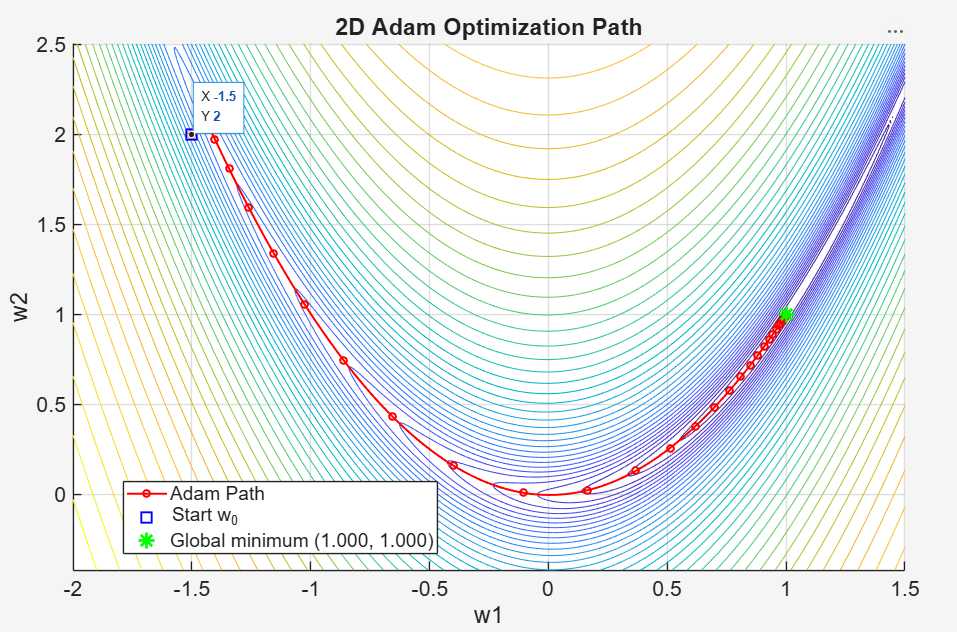
\includegraphics[width=0.78\textwidth]{figures/Beale_2D_Contour.png}
    \caption{Optimization trajectory of ADAM on the 2D Rosenbrock contour.}
    \label{fig:rosenbrock_contour}
\end{figure}

\begin{figure}[H]
    \centering
    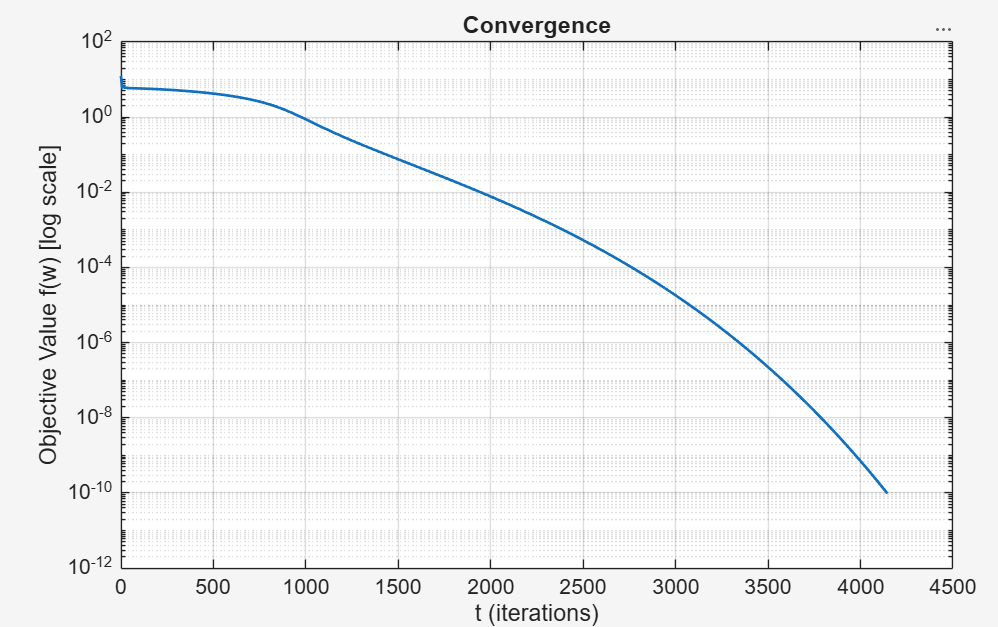
\includegraphics[width=0.78\textwidth]{figures/Beale_Convergence.png}
    \caption{Convergence history of the objective value $f(w_t)$ on logarithmic scale for the 2D Rosenbrock benchmark.}
    \label{fig:rosenbrock_convergence}
\end{figure}

\paragraph{Convergence Dynamics:}
ADAM quickly descends from the initial point $(-1.5, 2.0)$ into the parabolic ravine during the first $1{,}500$ iterations. It then steadily traverses the curved valley floor without oscillating across the steep walls, reaching the minimum $(1, 1)$ with high precision.

% -------------------------------------------------------------------------
\subsection{Beale Function}

\paragraph{Objective Function:}
The Beale function is defined as:
\begin{equation}
    f(x_1, x_2) = (1.5 - x_1 + x_1 x_2)^2 + (2.25 - x_1 + x_1 x_2^2)^2 + (2.625 - x_1 + x_1 x_2^3)^2
\end{equation}

\paragraph{Analytical Gradient:}
Differentiating $f$ with respect to $x_1$ and $x_2$ yields:
\begin{align}
    \frac{\partial f}{\partial x_1} &= 2x_1 x_2^6 + 2x_1 x_2^4 - 4x_1 x_2^3 - 2x_1 x_2^2 - 4x_1 x_2 + 6x_1 + \frac{21}{4}x_2^3 + \frac{9}{2}x_2^2 + 3x_2 - \frac{51}{4} \\
    \frac{\partial f}{\partial x_2} &= 6x_1^2 x_2^5 + 4x_1^2 x_2^3 - 6x_1^2 x_2^2 - 2x_1^2 x_2 - 2x_1^2 + \frac{63}{4}x_1 x_2^2 + 9x_1 x_2 + 3x_1
\end{align}

\paragraph{Global Minimum:}
The unique global minimum is located at $x^* = (3, 0.5)$ with $f(x^*) = 0$.

\begin{table}[H]
\centering
\caption{Hyperparameter Setup for 2D Beale Benchmark}\label{tab:beale_params}
\begin{tabular}{lc}
\toprule
\textbf{Parameter} & \textbf{Value} \\
\midrule
$w_0$ & $(1, 0)$ \\
$\alpha$ & $0.01$ \\
$\text{max\_iter}$ & $15{,}000$ \\
$\beta_1$ & $0.9$ \\
$\beta_2$ & $0.999$ \\
$\varepsilon$ & $1 \times 10^{-8}$ \\
$\text{tol}$ & $1 \times 10^{-5}$ \\
\bottomrule
\end{tabular}
\end{table}

\paragraph{Results \& Verification:}
ADAM converged to the global minimum in $2{,}491$ iterations, matching the Nelder-Mead benchmark from MATLAB's \texttt{fminsearch}.

\begin{table}[H]
\centering
\caption{Verification of Solution on Beale Function}\label{tab:beale_verif}
\begin{tabular}{lcc}
\toprule
\textbf{Method} & $x_1$ & $x_2$ \\
\midrule
Known minimum & $3.0000$ & $0.5000$ \\
ADAM optimizer & $3.0000$ & $0.5000$ \\
\texttt{fminsearch} verification & $3.0000$ & $0.5000$ \\
\bottomrule
\end{tabular}
\end{table}

\begin{figure}[H]
    \centering
    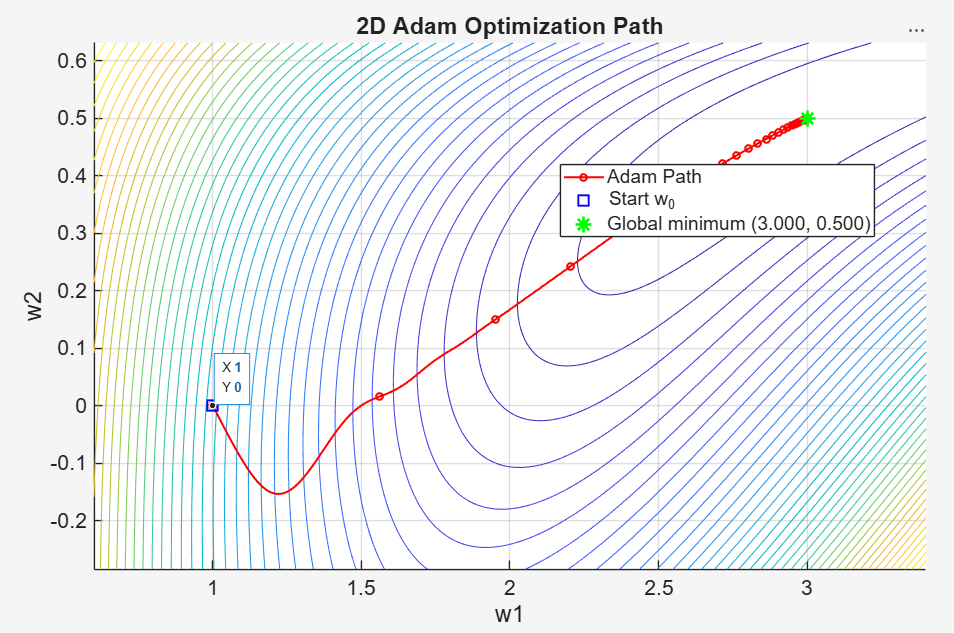
\includegraphics[width=0.78\textwidth]{figures/Rosenbrock_2D_Contour.png}
    \caption{Optimization trajectory of ADAM on the 2D Beale contour.}
    \label{fig:beale_contour}
\end{figure}

\begin{figure}[H]
    \centering
    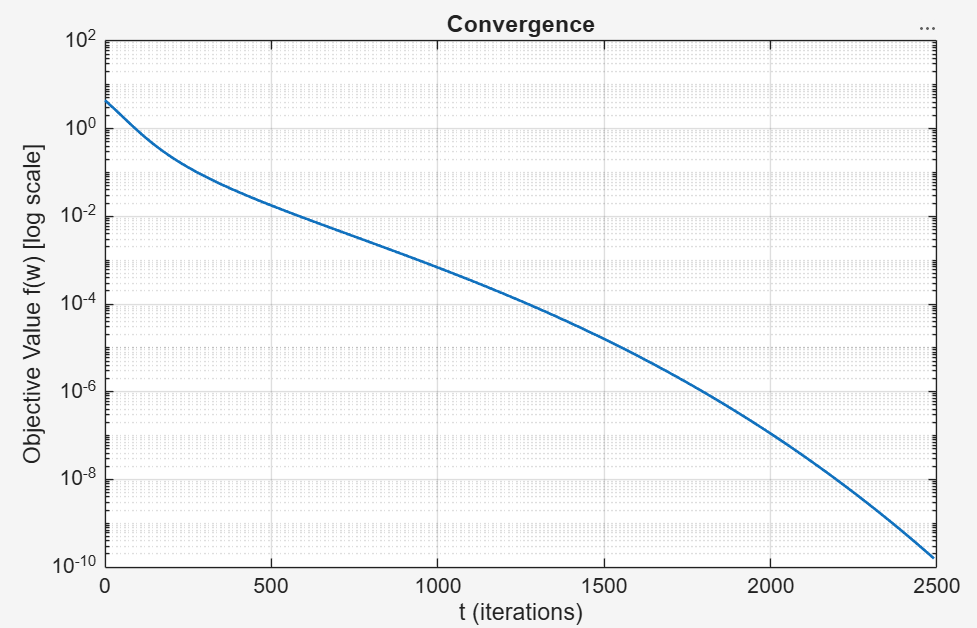
\includegraphics[width=0.78\textwidth]{figures/Rosenbrock_Convergence.png}
    \caption{Convergence history of the objective value $f(w_t)$ on logarithmic scale for the 2D Beale benchmark.}
    \label{fig:beale_convergence}
\end{figure}

\paragraph{Convergence Dynamics:}
Starting from $(1, 0)$, ADAM smoothly navigates the sharp contours and extended flat regions of the Beale surface, achieving steady logarithmic loss reduction down to the tolerance threshold at $(3, 0.5)$.

% =========================================================================
\section{Comparative Analysis: ADAM vs. Steepest Descent and Newton's Method}

To understand how ADAM behaves on curved, ill-conditioned valleys, we compare its trajectory on the 2D Rosenbrock function with two classical optimization methods:
\begin{itemize}
    \item \textbf{Steepest Descent}: Standard first-order method updating along $w_t = w_{t-1} - \alpha \nabla f(w_{t-1})$.
    \item \textbf{Newton's Method}: Second-order method utilizing the exact inverse Hessian $w_t = w_{t-1} - H^{-1}(w_{t-1})\nabla f(w_{t-1})$, with:
    \begin{equation}
        H(x_1, x_2) = \begin{bmatrix} 2 - 400 x_2 + 1200 x_1^2 & -400 x_1 \\ -400 x_1 & 200 \end{bmatrix}
    \end{equation}
    \item \textbf{ADAM}: First-order adaptive method combining momentum with coordinate-wise learning rate scaling.
\end{itemize}

All methods were evaluated from the same initial point $w_0 = (-1.5, 2.0)$ with a convergence tolerance of $\tau = 10^{-5}$.

\begin{table}[H]
\centering
\caption{Iteration Count Comparison on 2D Rosenbrock Function}\label{tab:rosenbrock_comp}
\begin{tabular}{lc}
\toprule
\textbf{Optimization Method} & \textbf{Iterations to Convergence} \\
\midrule
ADAM & $4{,}145$ \\
Steepest Descent & $13{,}821$ \\
Newton's Method & $5$ \\
\bottomrule
\end{tabular}
\end{table}

\begin{figure}[H]
    \centering
    \begin{subfigure}[b]{0.49\textwidth}
        \centering
        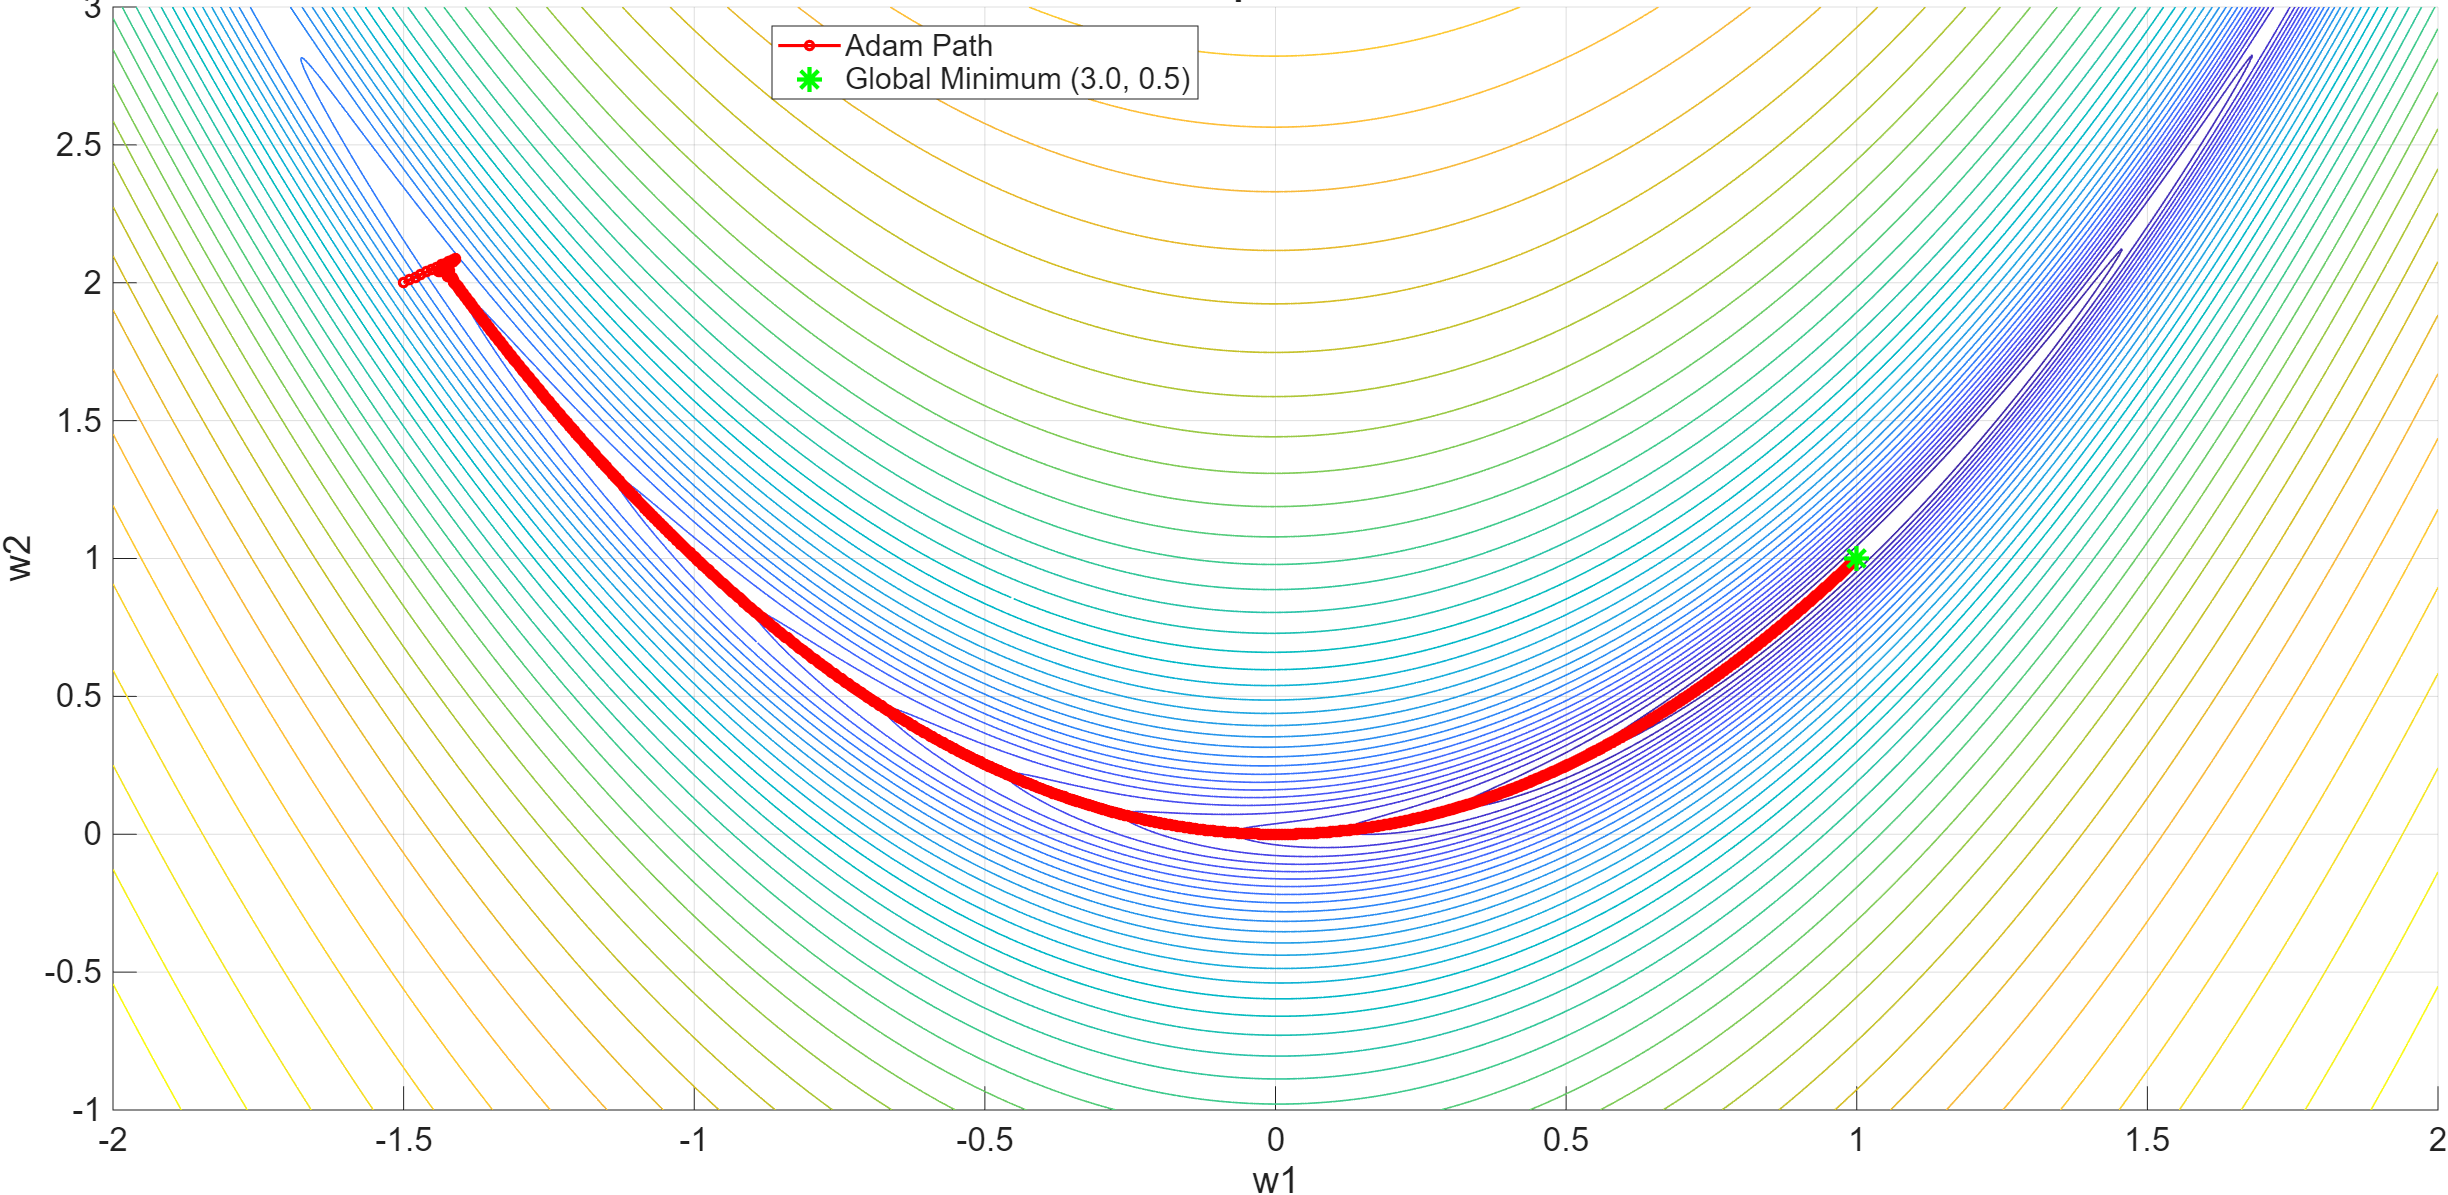
\includegraphics[width=\textwidth]{figures/ADAM_2D_Contour.png}
        \caption{ADAM}
    \end{subfigure}
    \hfill
    \begin{subfigure}[b]{0.49\textwidth}
        \centering
        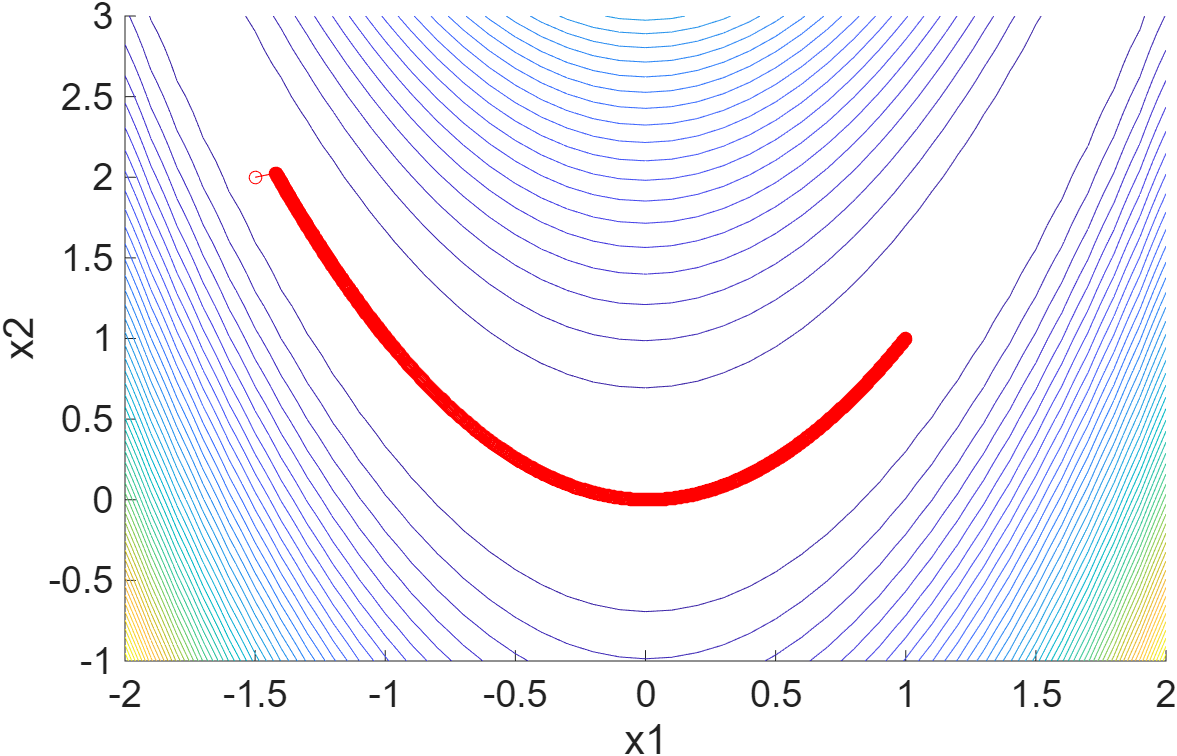
\includegraphics[width=\textwidth]{figures/Steepest_Descent_Rosenbrock.png}
        \caption{Steepest Descent}
    \end{subfigure}
    \vskip 0.8em
    \begin{subfigure}[b]{0.49\textwidth}
        \centering
        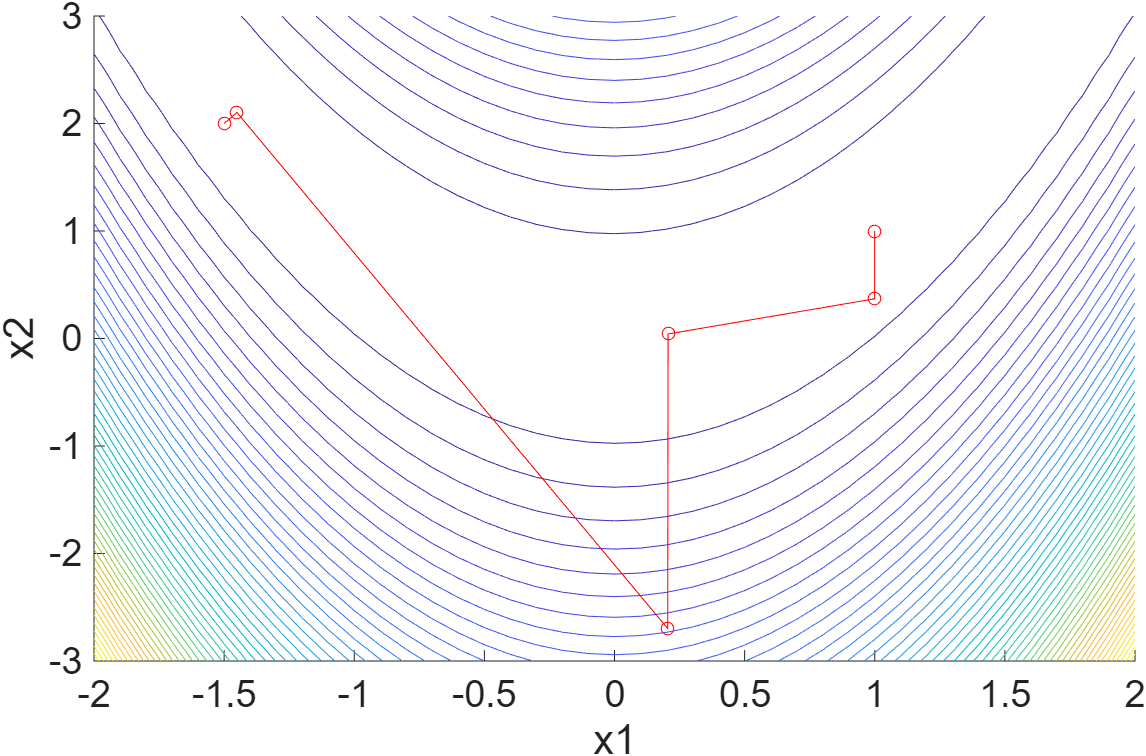
\includegraphics[width=\textwidth]{figures/Newton.png}
        \caption{Newton's Method}
    \end{subfigure}
    \hfill
    \begin{subfigure}[b]{0.49\textwidth}
        \centering
        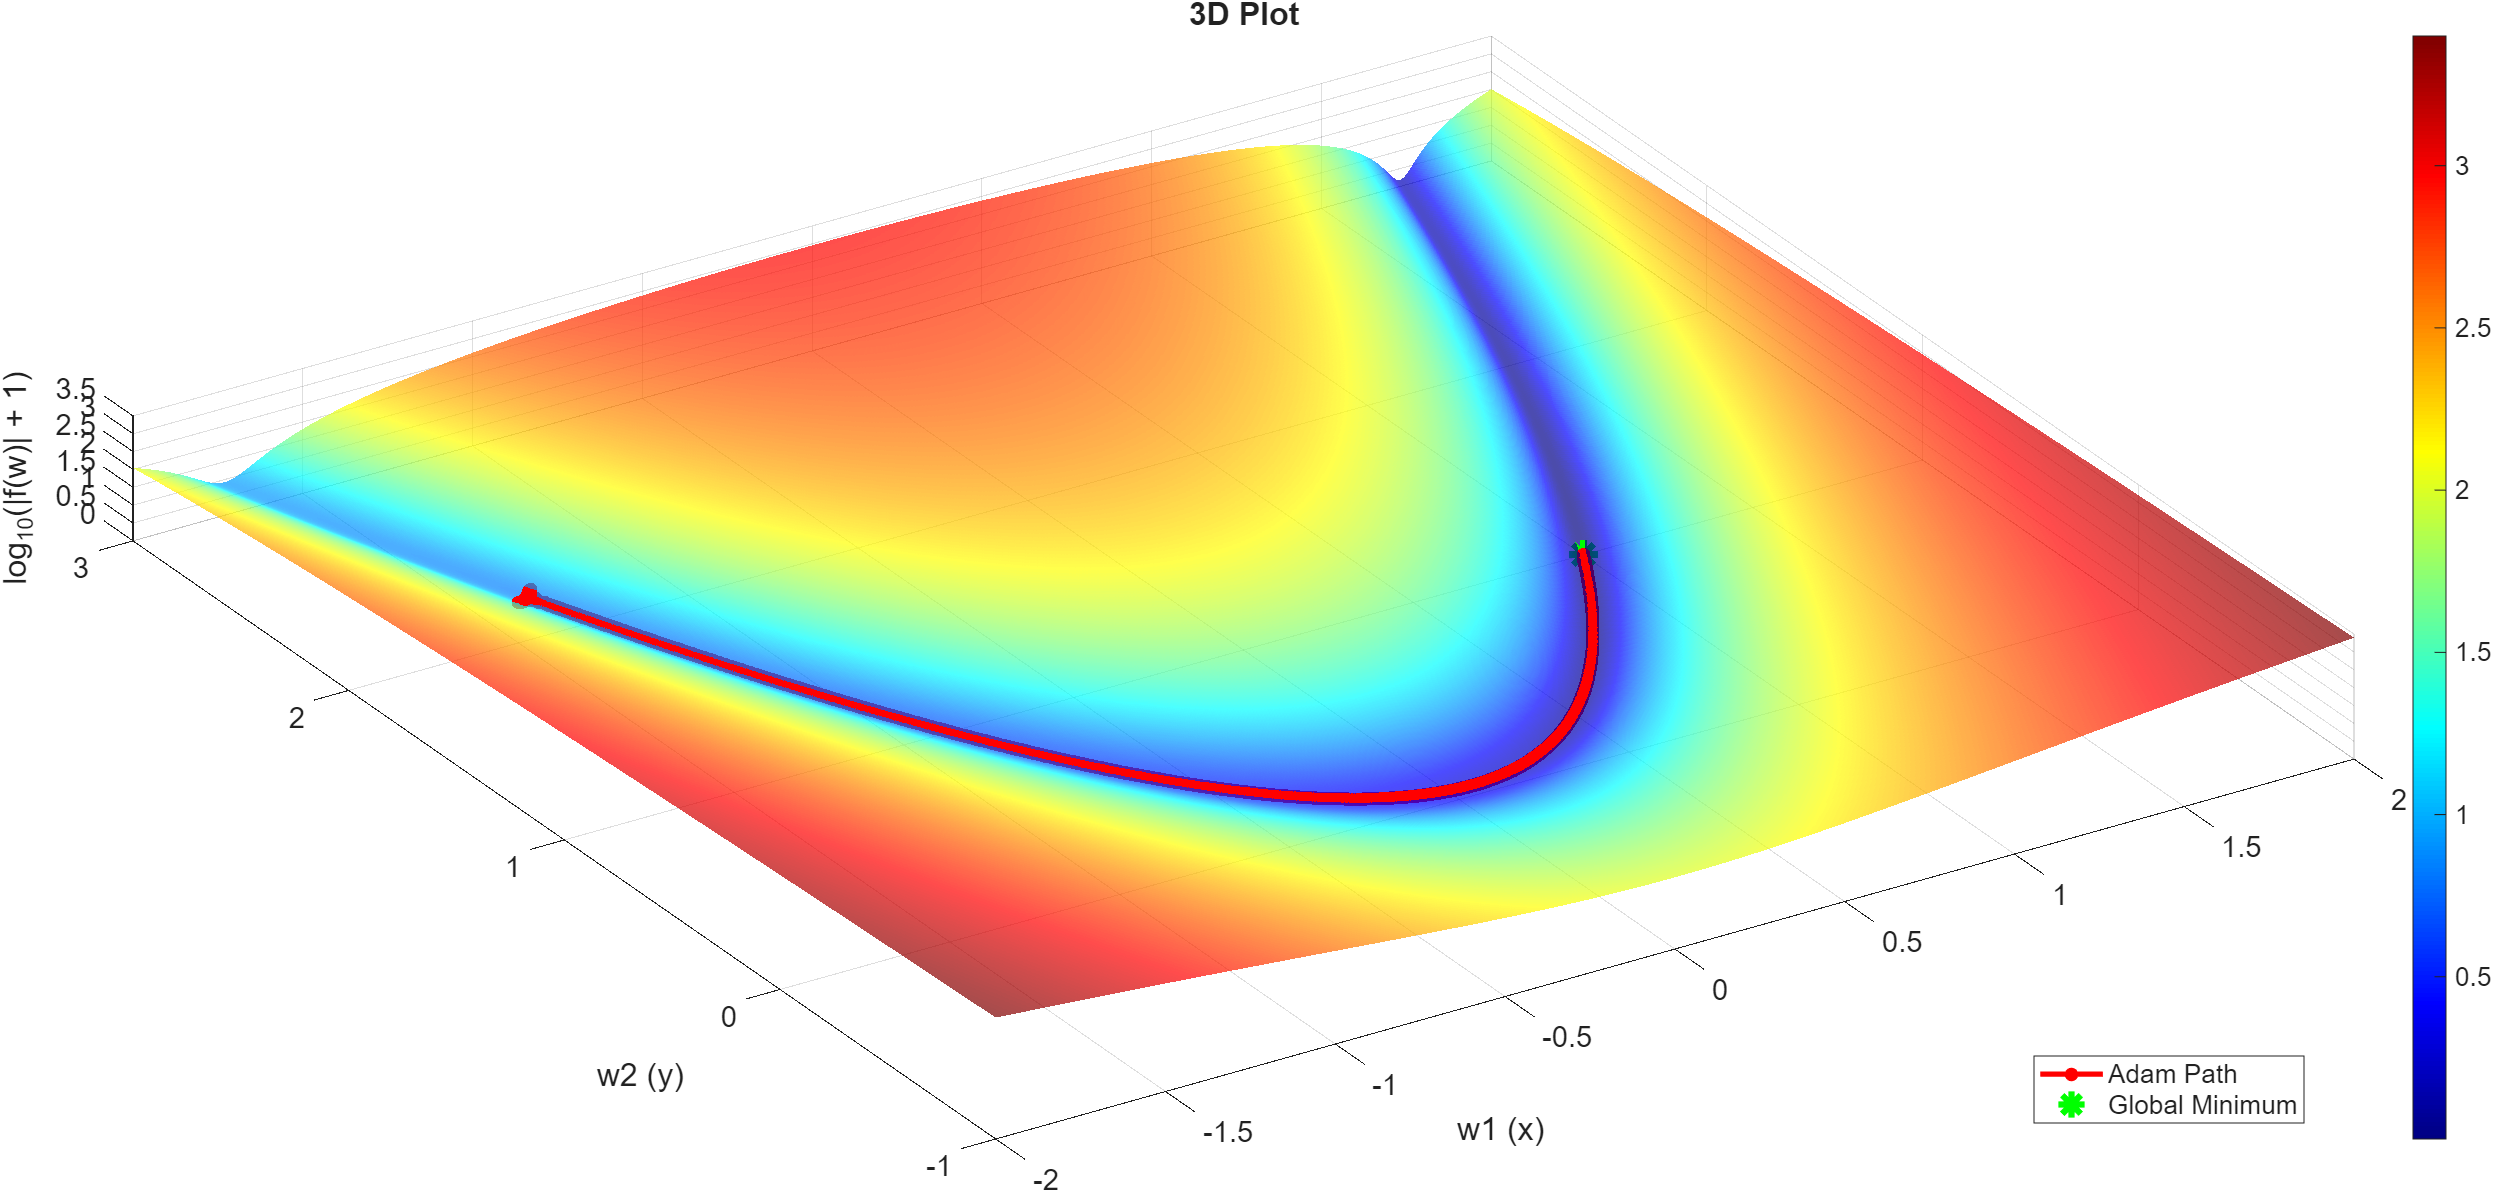
\includegraphics[width=\textwidth]{figures/3D_Surface_Plot.png}
        \caption{3D surface geometry}
    \end{subfigure}
    \caption{Optimization trajectories of ADAM, Steepest Descent, and Newton's Method on the 2D Rosenbrock contour, alongside the 3D surface geometry.}\label{fig:2d_comparison}
\end{figure}

\begin{itemize}
    \item \textbf{Steepest Descent} struggles because the gradient vectors are nearly perpendicular to the long valley floor. As a result, the iterates bounce back and forth between the steep valley walls, making slow progress along the bottom and taking $13{,}821$ iterations to converge.
    \item \textbf{ADAM} uses momentum to dampen these cross-valley oscillations while accelerating along the valley floor. Individual coordinate scaling adapts step sizes along each direction, navigating the curve smoothly in $4{,}145$ iterations without requiring second derivatives.
    \item \textbf{Newton's Method} uses exact curvature information from the Hessian matrix, finding the global minimum in only $5$ iterations. However, forming and inverting the $D \times D$ Hessian requires $\mathcal{O}(D^3)$ operations per step, which becomes computationally impractical for high-dimensional problems.
\end{itemize}

% =========================================================================
\section{Medium-Scale Benchmark: 100D Extended Rosenbrock}

\subsection{Formulation and Gradient Derivation}
Moving beyond 2D tests, we evaluate ADAM on a medium-scale benchmark by extending the Rosenbrock function to $D = 100$ design variables:
\begin{equation}
    f(w) = \sum_{i=1}^{D-1} \left[ 100 (w_{i+1} - w_i^2)^2 + (1 - w_i)^2 \right], \quad w \in \mathbb{R}^D
\end{equation}
The global minimum is located at $w^* = (1, 1, \dots, 1)^T$ with $f(w^*) = 0$.

\noindent The exact analytical gradient components $\nabla f(w) = [\frac{\partial f}{\partial w_1}, \dots, \frac{\partial f}{\partial w_D}]^T$ are derived as:
\begin{align}
    \frac{\partial f}{\partial w_1} &= -400 w_1 (w_2 - w_1^2) - 2(1 - w_1) \\
    \frac{\partial f}{\partial w_i} &= 200 (w_i - w_{i-1}^2) - 400 w_i (w_{i+1} - w_i^2) - 2(1 - w_i), \quad \text{for } 2 \le i \le D-1 \\
    \frac{\partial f}{\partial w_D} &= 200 (w_D - w_{D-1}^2)
\end{align}

\subsection{Simulation Setup}
The experiment is executed via \texttt{adam\_runner\_100D\_extended\_rosenbrock\_func.m} with the following configuration:
\begin{itemize}
    \item Dimension: $D = 100$
    \item Initial Guess: $w_0 = [-1.5, 2.0, -1.5, 2.0, \dots]^T \in \mathbb{R}^{100}$
    \item Hyperparameters: $\alpha = 0.005$, $\beta_1 = 0.9$, $\beta_2 = 0.999$, $\varepsilon = 10^{-8}$, $\tau = 10^{-5}$
    \item Maximum Iterations: $25{,}000$
\end{itemize}

\subsection{Empirical Results \& Convergence Dynamics}

\begin{figure}[H]
    \centering
    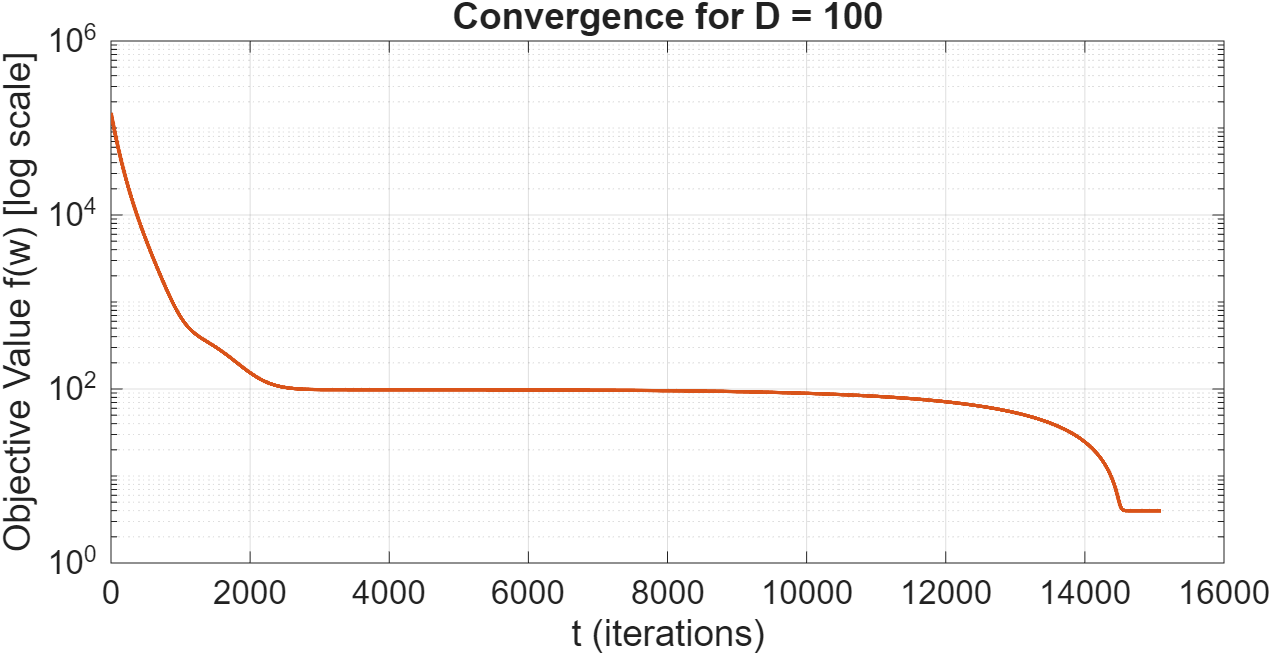
\includegraphics[width=0.78\textwidth]{figures/Convergence_f_w.png}
    \caption{Objective function convergence history on logarithmic scale for the 100D Extended Rosenbrock benchmark.}\label{fig:100d_loss}
\end{figure}

\begin{figure}[H]
    \centering
    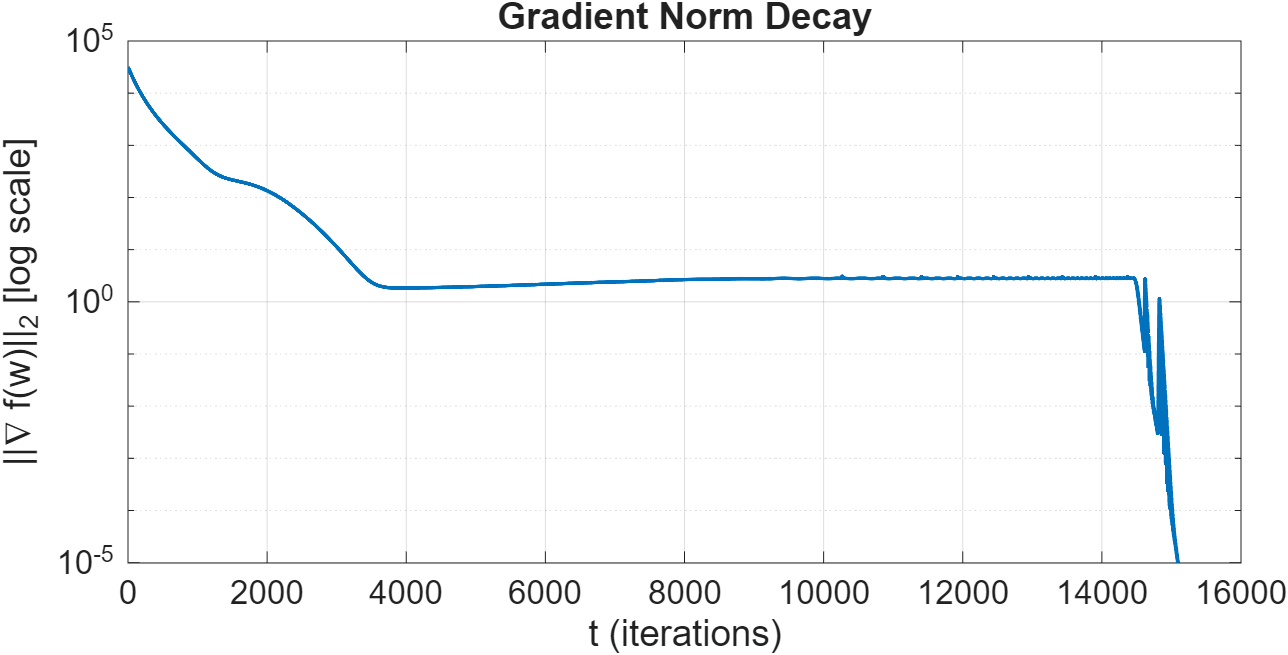
\includegraphics[width=0.78\textwidth]{figures/Gradient_Norm_Convergence.png}
    \caption{Gradient norm decay $\|\nabla f(w_t)\|_2$ during optimization of the 100D Extended Rosenbrock problem.}\label{fig:100d_grad}
\end{figure}

\begin{figure}[H]
    \centering
    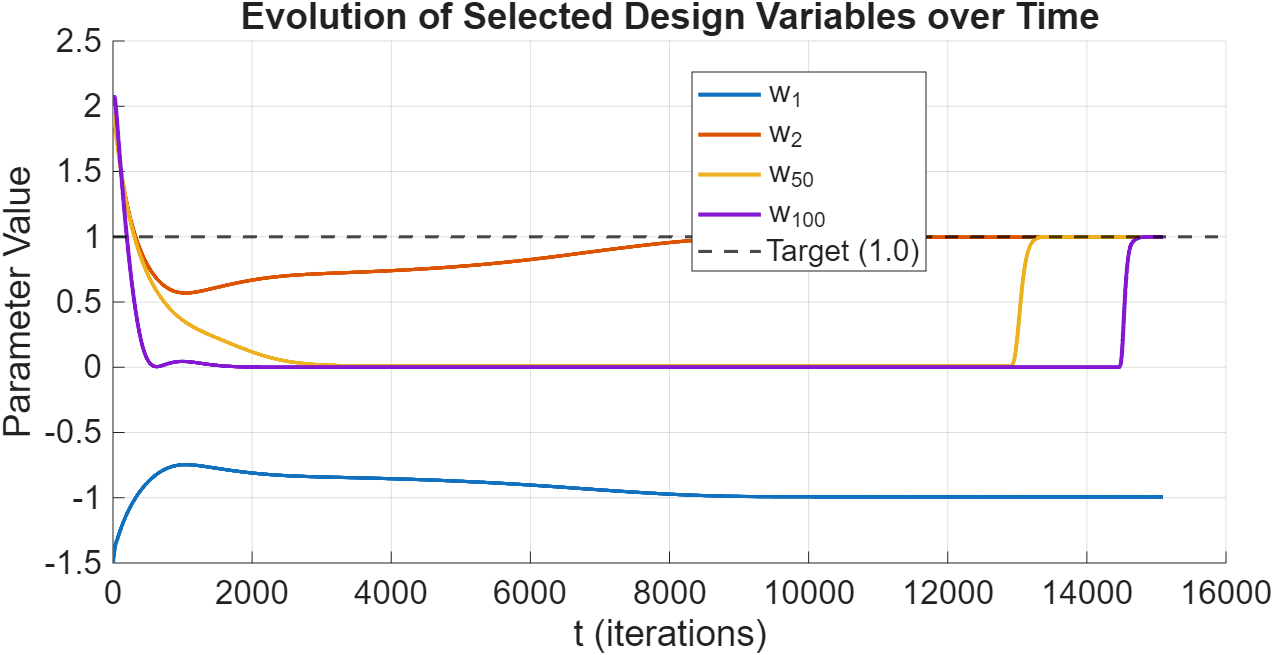
\includegraphics[width=0.78\textwidth]{figures/Selected_Coordinate_Trajectories.png}
    \caption{Evolution of selected design variables ($w_1, w_2, w_{50}, w_{100}$) during optimization of the 100D Extended Rosenbrock benchmark.}\label{fig:100d_trajectories}
\end{figure}

\begin{table}[H]
\centering
\caption{Empirical Convergence Metrics for 100D Extended Rosenbrock Optimization}\label{tab:100d_metrics}
\begin{tabular}{lc}
\toprule
\textbf{Metric} & \textbf{Observed Value} \\
\midrule
Iterations to Convergence & $15{,}094$ \\
Computation Time & $0.96\text{ seconds}$ \\
Final Objective Value $f(w^*)$ & $3.986624 \times 10^{0}$ \\
$\ell_2$-Distance to Global Minimum $\|w^* - w_{\text{global}}\|_2$ & $1.993290 \times 10^{0}$ \\
Gradient Norm at Convergence $\|\nabla f(w^*)\|_2$ & $9.851188 \times 10^{-6}$ (satisfies $\tau \le 10^{-5}$) \\
Design Variable Range $[\min(w^*), \max(w^*)]$ & $[-0.9933, 1.0000]$ \\
\bottomrule
\end{tabular}
\end{table}

\begin{itemize}
    \item \textbf{Objective Decay:} As shown in Figure~\ref{fig:100d_loss}, the objective function exhibits a steep initial descent followed by steady logarithmic progress as ADAM traverses the 100-dimensional valley, reaching $f(w^*) = 3.9866$ within $0.96$ seconds ($15{,}094$ iterations).
    \item \textbf{Gradient Norm:} Figure~\ref{fig:100d_grad} confirms stable convergence to the specified gradient norm tolerance $\|\nabla f(w)\|_2 = 9.85 \times 10^{-6} \le 10^{-5}$ without oscillations or numerical divergence.
    \item \textbf{Coordinate Dynamics:} Figure~\ref{fig:100d_trajectories} tracks early ($w_1, w_2$), intermediate ($w_{50}$), and boundary ($w_{100}$) variables, illustrating coordinated convergence across all 100 dimensions.
\end{itemize}

\added{\subsection{Comparative Benchmark of Modern ADAM Variants}}

\added{To investigate algorithmic behavior across different optimizer formulations, we evaluated five variants on the same 100-dimensional Extended Rosenbrock benchmark ($w_0 = [-1.5, 2.0, \dots]^T$, $\alpha = 0.005$, $\beta_1 = 0.9$, $\beta_2 = 0.999$, $\varepsilon = 10^{-8}$, $\tau = 10^{-5}$, max iterations $25{,}000$). Table~\ref{tab:100d_variants_benchmark} summarizes the empirical performance metrics.}

\added{\begin{table}[H]
\centering
\small
\setlength{\tabcolsep}{5pt}
\caption{Benchmark Comparison of ADAM Variants on 100D Extended Rosenbrock}\label{tab:100d_variants_benchmark}
\begin{tabular}{lccccc}
\toprule
\textbf{Optimizer} & \textbf{Iterations} & \textbf{Time (s)} & $f(w^*)$ & $\|w^* - w^*_{\text{global}}\|_2$ & $\|\nabla f(w^*)\|_2$ \\
\midrule
ADAM & $15{,}094$ & $0.11$ & $3.9866$ & $1.9933$ & $9.85 \times 10^{-6}$ \\
AdamW ($\lambda = 0.1$) & $25{,}000$ & $0.16$ & $\mathbf{0.0024}$ & $\mathbf{0.0527}$ & $2.3474$ \\
AMSGrad & $25{,}000$ & $0.16$ & $98.3683$ & $9.9052$ & $3.4744$ \\
ADAM-DG (Hypergradient) & $\mathbf{8{,}736}$ & $\mathbf{0.07}$ & $3.9866$ & $1.9933$ & $9.18 \times 10^{-6}$ \\
Preconditioned ADAM & $25{,}000$ & $0.91$ & $3.9874$ & $1.9933$ & $1.4066$ \\
\bottomrule
\end{tabular}
\end{table}}

\added{\paragraph{Analysis of Convergence Characteristics:}
\begin{itemize}
    \item \textbf{Local Minimum Basin vs. Saddle Point (ADAM \& ADAM-DG):} Both standard ADAM and ADAM-DG successfully satisfied the gradient convergence tolerance $\tau = 10^{-5}$, settling at $w_1^* = -0.9933$ and $w_i^* = 1.0000$ for $i \ge 2$, with $f(w^*) \approx 3.9866$. Spectral analysis confirms that all $100$ eigenvalues of the Hessian at this point are strictly positive, ranging from $\lambda_{\min} \approx 0.499$ to $\lambda_{\max} \approx 1801.6$. This proves that the optimizers converged to a genuine, highly flat local minimum basin rather than stalling at a saddle point, matching the theoretical stationary point analysis of Kok and Sandrock \cite{kok2009locating}.
    \item \textbf{Decoupled Weight Decay Mechanics (AdamW):} AdamW \cite{loshchilov2017decoupled} reached the lowest objective value ($f = 0.0024$) and closest distance to the global minimum ($\|w^* - w^*_{\text{global}}\|_2 = 0.0527$). However, it reached the iteration limit because the gradient norm remained at $2.3474$. In AdamW, parameter updates include a direct decay term $-\alpha \lambda w_t$ independent of the gradient. Consequently, equilibrium occurs where the objective gradient balances the regularization pull ($\nabla f(w) \approx \lambda w$), meaning $\|\nabla f(w)\|_2$ does not vanish to zero.
    \item \textbf{Denominator Saturation and Freezing (AMSGrad):} AMSGrad \cite{reddi2018convergence} failed to traverse the valley, stalling at $f = 98.3683$ with coordinates $w_6$ through $w_{100}$ remaining near their starting values. Because AMSGrad enforces $\hat{v}_t = \max(\hat{v}_{t-1}, v_t)$, large initial gradient spikes permanently inflated the denominator, suppressing effective step sizes for the remainder of the run.
\end{itemize}}

% =========================================================================
\added{\section{Advanced Gradient Dynamics and Curvature Preconditioning}}

\added{\subsection{Double Gradient Descent via Hypergradient Adaptation}}

\added{Standard ADAM relies on a fixed, manually tuned learning rate $\alpha$. Double gradient descent (hypergradient descent) \cite{baydin2018online} formulates the stepsize $\alpha$ itself as an optimization parameter, updating it at each iteration via gradient descent on the objective function with respect to $\alpha$:}
\added{\begin{equation}
    \alpha_t = \alpha_{t-1} - \beta_h \frac{\partial f(w_{t-1})}{\partial \alpha_{t-1}}
\end{equation}}
\added{Applying the chain rule yields:}
\added{\begin{equation}
    \frac{\partial f(w_{t-1})}{\partial \alpha_{t-1}} = \nabla f(w_{t-1})^T \frac{\partial w_{t-1}}{\partial \alpha_{t-1}} = -\nabla f(w_{t-1})^T u_{t-2}
\end{equation}}
\added{where $u_{t-2} = \hat{m}_{t-2} \oslash (\sqrt{\hat{v}_{t-2}} + \varepsilon)$ is the previous ADAM update direction and $\beta_h$ is the hypergradient learning rate. Intuitively, if the current gradient aligns with the previous update vector ($\nabla f(w_{t-1})^T u_{t-2} > 0$), the optimizer increases $\alpha_t$ to accelerate progress along the valley. Conversely, if the vectors oppose each other, it decreases $\alpha_t$ to prevent overshooting. On the 100D Extended Rosenbrock problem, this adaptive mechanism reduced the required iterations from $15{,}094$ to $8{,}736$ (a $42.1\%$ reduction) while reaching the exact same local minimum.}

\added{\begin{figure}[H]
    \centering
    \begin{subfigure}[b]{0.48\textwidth}
        \centering
        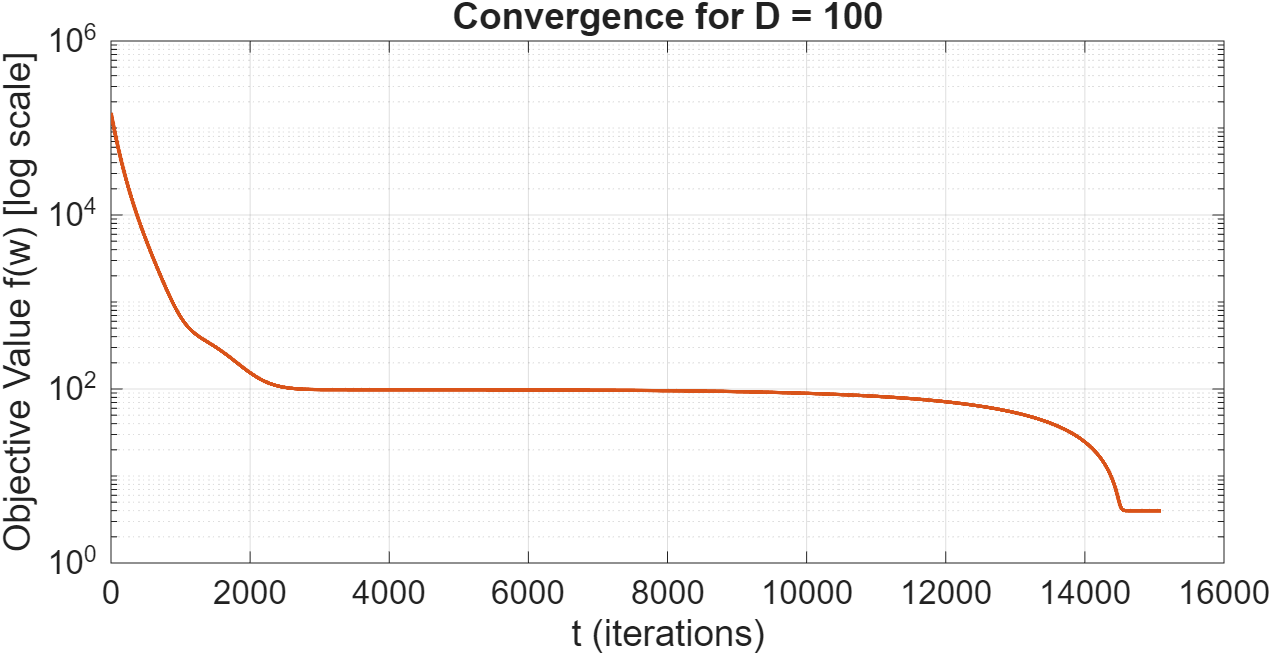
\includegraphics[width=\textwidth]{figures/Convergence_f_w.png}
        \caption{Standard ADAM ($15{,}094$ iterations)}
    \end{subfigure}
    \hfill
    \begin{subfigure}[b]{0.48\textwidth}
        \centering
        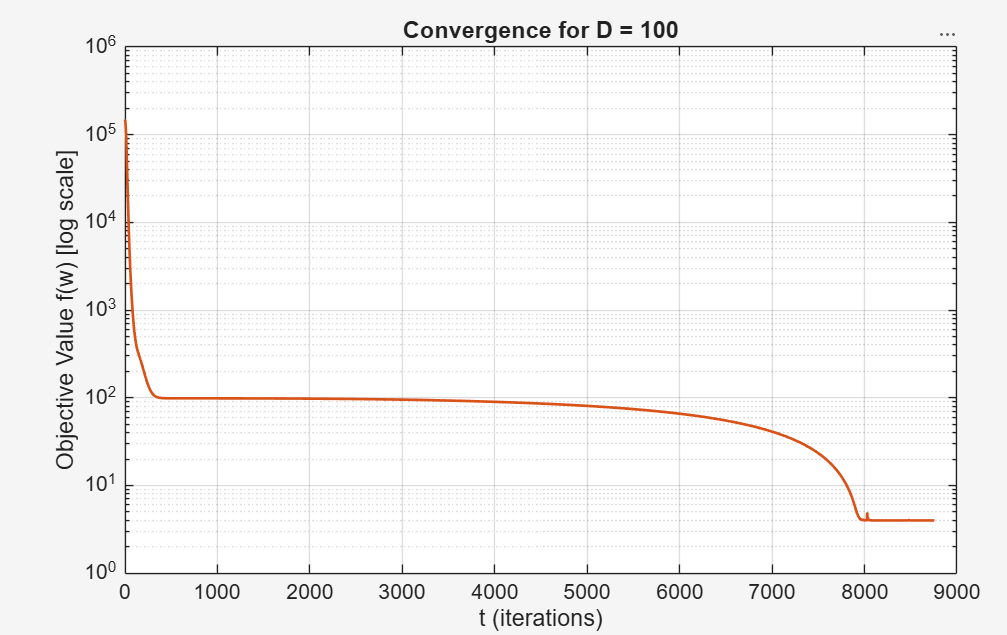
\includegraphics[width=\textwidth]{figures/Convergence_f_w_DG.png}
        \caption{ADAM-DG ($8{,}736$ iterations)}
    \end{subfigure}
    \caption{Comparison of objective function convergence on logarithmic scale between Standard ADAM and ADAM with Double Gradient (Hypergradient Descent) on the 100D Extended Rosenbrock benchmark.}\label{fig:adam_vs_dg_convergence}
\end{figure}}

\added{\subsection{Stabilized Curvature Preconditioning}}

\added{While first-order ADAM uses coordinate-wise scaling $\sqrt{\hat{v}_t}$, it treats parameter dimensions independently. Curvature preconditioning transforms the gradient by an approximation of the inverse Hessian matrix before computing moment estimates:}
\added{\begin{equation}
    p_t = H^{-1}(w_t) \nabla f(w_t)
\end{equation}}
\added{On non-convex objective landscapes, raw Newton steps can diverge because the Hessian $H(w)$ is not positive definite away from stationary points, causing $H^{-1} \nabla f$ to point uphill. To ensure numerical stability, our implementation incorporates two safeguards based on Nocedal and Wright \cite{nocedal2006numerical}:}
\added{\begin{enumerate}
    \item \textbf{Adaptive Diagonal Regularization:} We compute the Cholesky factorization of $H + \tau I$. If factorization fails (indicating non-positive definiteness), the regularization parameter $\tau$ is iteratively increased by factors of $10$ until positive definiteness is restored.
    \item \textbf{Descent Direction Verification:} Before updating, we check the condition $\nabla f(w_t)^T p_t > 0$. If this test fails, the algorithm discards the preconditioned direction and falls back to the steepest descent gradient $\nabla f(w_t)$.
\end{enumerate}}
\added{To avoid analytical second derivatives, the Hessian entries are estimated numerically via central differences of the gradient. To maintain computational efficiency, the preconditioning matrix is refreshed every $50$ iterations while testing the descent direction condition at every step, reducing computation time to $0.91$ seconds.}

\added{\subsection{Black-Box / Zeroth-Order Gradient Estimation}}

\added{For optimization problems where analytical gradients are unavailable (e.g., external simulation software or experimental systems), the gradient vector can be approximated using function evaluations alone:}
\added{\begin{itemize}
    \item \textbf{Central Finite Differences (CFD):} Evaluates symmetric perturbations along each coordinate:
    \begin{equation}
        g_i \approx \frac{f(w + h e_i) - f(w - h e_i)}{2h}, \quad i = 1, \dots, D
    \end{equation}
    CFD achieves $\mathcal{O}(h^2)$ truncation accuracy but requires $2D$ function calls per step.
    \item \textbf{Simultaneous Perturbation Stochastic Approximation (SPSA):} Perturbs all $D$ variables simultaneously with a random vector $\Delta \in \mathbb{R}^D$ (e.g., Rademacher $\pm 1$):
    \begin{equation}
        \hat{g} \approx \frac{f(w + h \Delta) - f(w - h \Delta)}{2h} \Delta^{-1}
    \end{equation}
    SPSA requires only $2$ function evaluations per step regardless of dimension $D$. The stochastic perturbation noise is subsequently smoothed by ADAM's momentum accumulator $m_t$.
\end{itemize}}

% =========================================================================
\section{Future Research and Development Plans}

We plan to extend our MATLAB optimization framework in the following directions:
\begin{itemize}
    \item \added{\textbf{Stochastic Mini-Batch Analysis:} Benchmarking ADAM-DG and AdamW under stochastic noise to evaluate variance adaptation on non-deterministic loss landscapes.}
    \item \added{\textbf{High-Dimensional Scaling ($D = 10^3 \dots 10^5$):} Implementing matrix-free Hessian-vector products ($H v \approx \frac{\nabla f(w + \delta v) - \nabla f(w)}{\delta}$) to capture directional curvature at large dimensions without forming full matrices.}
    \item \textbf{Neural Network Training with Adjoint Gradients:} Train linear and non-linear networks in MATLAB, using LU decomposition ($\mathbf{A} = \mathbf{L}\mathbf{U}$) and the adjoint state method to compute gradients efficiently for regression and MNIST.
    \item \added{\textbf{Uncertainty Quantification in Optimization:} Linking ADAM's adaptive variance vector $v_t$ with stochastic sensitivity estimation for structural reliability problems.}
\end{itemize}

% =========================================================================
\bibliographystyle{plain}
\bibliography{references}

\end{document}
